\documentclass{article}
    % General document formatting
    \usepackage[margin=0.7in]{geometry}
    \usepackage[parfill]{parskip}
    \usepackage{amsopn}
    \usepackage{mathtools}
    \usepackage[utf8]{inputenc}
    \usepackage{hyperref}
    \usepackage{multicol}
    \usepackage{amsmath,amssymb,amsfonts,amsthm}
    \usepackage{dot2texi}
    \usepackage{tikz}
    \usetikzlibrary{shapes,arrows}

    \DeclareMathOperator{\StringT}{StringT}
    \DeclareMathOperator{\NumberT}{NumberT}
    \DeclareMathOperator{\BooleanT}{BooleanT}
    \DeclareMathOperator{\LitT}{LitT}
    \DeclareMathOperator{\JSLit}{JSLit}
    \DeclareMathOperator{\JSTypeof}{JSTypeof}
    \DeclareMathOperator{\RecT}{RecT}
    \DeclareMathOperator{\ObjT}{ObjT}
    \DeclareMathOperator{\ListT}{ListT}
    \DeclareMathOperator{\SetT}{SetT}
    \DeclareMathOperator{\MapT}{MapT}
    \DeclareMathOperator{\ObjType}{ObjType}
    \DeclareMathOperator{\UnionT}{UnionT}
    \DeclareMathOperator{\InterT}{InterT}
    \DeclareMathOperator{\LookupObjRef}{LookupObjRef}
    \DeclareMathOperator{\String}{String}
    \DeclareMathOperator{\Number}{Number}
    \DeclareMathOperator{\Boolean}{Boolean}
    \DeclareMathOperator{\type-ref}{ref}
    \DeclareMathOperator{\Type}{Type}
    \DeclareMathOperator{\NoSuper}{NoSuper}
    \DeclareMathOperator{\InterOrObj}{InterOrObj}
    \DeclareMathOperator{\ObjectSubtype}{ObjectSubtype}
    \DeclareMathOperator{\RecordSubtype}{RecordSubtype}
    \DeclareMathOperator{\Value}{Value_\Sigma}
    \DeclareMathOperator{\StringV}{StringV_\Sigma}
    \DeclareMathOperator{\NumberV}{NumberV_\Sigma}
    \DeclareMathOperator{\BooleanV}{BooleanV_\Sigma}
    \DeclareMathOperator{\RecV}{RecV_\Sigma}
    \DeclareMathOperator{\ObjV}{ObjV_\Sigma}
    \DeclareMathOperator{\ListV}{ListV_\Sigma}
    \DeclareMathOperator{\SetV}{SetV_\Sigma}
    \DeclareMathOperator{\MapV}{MapV_\Sigma}
    \DeclareMathOperator{\UnionV}{UnionV_\Sigma}
    \DeclareMathOperator{\ValueType}{ValueType_\Sigma}
    \DeclareMathOperator{\textref}{ref}
    \DeclareMathOperator{\ObjFields}{ObjFields}
    \DeclareMathOperator{\ObjPairsMatch}{ObjPairsMatch}
    \DeclareMathOperator{\where}{ where }
    \DeclareMathOperator{\textif}{ if }
    \DeclareMathOperator{\suchthat}{s.t.}
    \newcommand{\ValueRef}{\textref}
    \newcommand{\ValueDeref}[1]{\Sigma(#1)}
\begin{document}

\title{Sinap's Type System}
\author{Sheyne Anderson}
\maketitle
\section{Intro}

\textbf{change voice to ``We"}

Sinap IDE is a program to allow editing of graph
programs in various graph programming langauages. 
Because it wants to be an editor for many different
graph-languages, a pluggable architecture was designed
so that Sinap could change its user interface (UI)
to best support each language. 

The idea is that while editing a graph, components of the
graph will have different attributes associated with them 
that the editor should present contextually. For example, in
a graph-language describing deterministic finite-state 
automata (DFAs) edges should have a ``symbol" attribute of 
type character corresponding to the input by which this 
edge should be followed. 

\begin{figure}[h]
    \label{sinap-screenshot}  
    \centering
    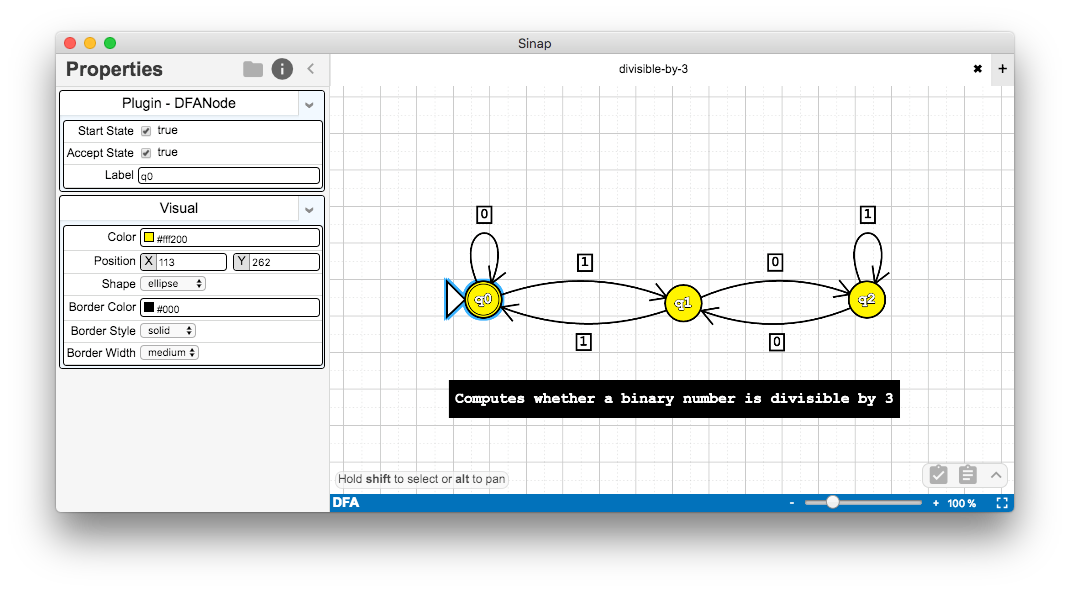
\includegraphics[width=.8\textwidth]{sinap-screenshot}
    \caption{Sinap IDE editing a graph}
\end{figure}

As you can see in Figure \ref{sinap-screenshot}, Sinap's UI
presents the user with nodes and edges which can be selected 
and edited in the sidebar. Allowing the sidebar to change based
on what interpreter is what the type-system facilitates. 
    
Sinap's type–system consists of two parts:

\begin{enumerate}
    \item A data-language to describe graph components 
    (implemented in values.ts)
    \item A data-description language to define valid schema 
    (implemented in types.ts)
    for the data language
\end{enumerate}

The code for both can be found at 

\href{https://github.com/2graphic/sinap-types}
{https://github.com/2graphic/sinap-types}.

The data that are allowable in the sidebar can be more complicated than
simple strings and numbers. In the example above the ``Position" attribute
of the node has a structure that similar to the following TypeScript code:

\begin{samepage}
\begin{verbatim}
type Point = {
    x: number;
    y: number;
}
\end{verbatim}
\end{samepage}

Although there fields aren't limited to simple types and the 
whole structure can nest. \textbf{TODO: awkward phrasing, reword}. 

\subsection{Notation}
\textbf{TODO: Matt: Do I want to keep this section at all? If so,
how should I expand it? Do I want to move the discussion 
of \(\Sigma\) to here?}

The symbol \((\operatorname{Kind}_1, ...)\) is equivalent to 
\((\operatorname{Kind}_i)\). They are also equivalent to 
\((\operatorname{Kind}_1, ..., \operatorname{Kind}_n)\)
where \(n\) is unspecified and represent an ordered list 
of \(n\) elements. \(\{\operatorname{Kind}_i\}\) represents 
the set of the elements of the list. 

``\(\_\)'' represents a symbol that has been omitted for brevity.

\textbf{Discuss the model here}

\section{The Type System}

\textbf{Move up}
\textbf{TODO: edit this next paragraph}
The goal of creating the above language (referred to as Sinap's 
Type System) is to allow interpreter implementers to specify what 
kinds of graphs are valid for their interpreter. This means that 
graphs can allow various fields on nodes and edges and the interpreter
can guarantee that the fields are present on all of the nodes that it
is passed. It also allows different kinds of nodes and edges to be 
specified and for rules to exists defining what kinds of nodes can 
via which edges. 


The data-description language is called the type system and has 
the following structure:

\begin{align*}
\begin{aligned}
\Type = &\LitT(\JSLit) \\
&|\StringT \\
&|\NumberT \\
&|\BooleanT \\
&|\RecT((\String, \Type), ...) \\
&|\ListT(\Type) \\
&|\SetT(\Type) \\
&|\MapT(\Type, \Type) \\
&|\ObjT\left(\begin{aligned}
    &\String, \String | \NoSuper, \\
&((\String, \Type), ...)
\end{aligned}\right) \\
&|\InterT(\ObjT, ...) \\
&|\UnionT(\Type, ...)\\
\end{aligned}
\quad\quad\quad\begin{aligned}        
\begin{aligned}
\JSLit = &\operatorname{JSString} \\
&| \operatorname{JSNumber} \\
&| \operatorname{true} \\
&| \operatorname{false} \\
\end{aligned}\\\\
\begin{aligned}
\JSTypeof(\operatorname{JSString}) &= \StringT \\
\JSTypeof(\operatorname{JSNumber}) &= \NumberT \\
\JSTypeof(\operatorname{true}) &= \BooleanT \\
\JSTypeof(\operatorname{false}) &= \BooleanT \\
\end{aligned}  
\end{aligned}  
\end{align*}


\textbf{TODO: motivate \(\LitT\)}
\textbf{TODO: motivate \(\InterT\)}
\textbf{Put above in figure? Walk though the figures again in prose}

\subsection{Subtype Relations}

\textbf{TODO: specifically \(\Gamma\) maps strings to object types}
\textbf{TODO: parameterize <: over \(\Gamma\)}
Define \(\bullet<:\bullet\)

\begin{align*}
    \Type_1&<:\Type_1 \\
    \LitT(\JSLit_1)&<:\Type_1 &&\textif \JSTypeof(\JSLit_1) = \Type_1 \\
    \InterT(\Type_{1,1}, ..., \Type_{1,n})&<:\InterT(\Type_{2,1}, ..., Type_{2,m}) 
    &&\textif \forall T\in \{\Type_{2,i}\} \exists T' \in \{\Type_{1,i}\} \suchthat T'<:T \\
    \InterT(..., \Type_i, ...)&<:\ObjT_1 &&\textif \ObjT_1 = \Type_i  \\
    \ObjT_1 &<: \ObjT(\String_1, \_, \_) &&\textif \ObjectSubtype(\String_1, \ObjT_1)\\
    \RecT_1&<:\RecT_2 &&\textif \RecordSubtype(\RecT_1, \RecT_2) \\
    \ListT(\Type_1)&<:\ListT(\Type_2) &&\textif \Type_1<:\Type_2 \\
    \SetT(\Type_1)&<:\SetT(\Type_2) &&\textif \Type_1<:\Type_2 \\
    \MapT(\Type_{11}, \Type_{12})&<:\MapT(\Type_{21}, \Type_{22}) &&\textif \Type_{11}<:\Type_{21} \text{ and } \Type_{12}<:\Type_{22} \\
\end{align*}
\begin{align*}
    \ObjectSubtype(\String_1, \ObjT(\String_2,\_, \_)) \quad &\textif 
    \quad (\String_1 = \String_2)\\
    \ObjectSubtype(\String_1, \ObjT(\_,\String_2, \_)) \quad &\textif 
    \quad \ObjectSubtype(\String_1, \LookupObjRef(\String_2)))
\end{align*}
\begin{align*}
    \RecordSubtype(\RecT((\String_{1,1}, \Type_{1, 1}), ..., (\String_{1,n}, \Type_{1, n})), \RecT((\String_{2,1}, \Type_{2, 1}), ..., (\String_{2,m}, \Type_{2, m}))) \\
    \textif \{\String_{2,i}\} \subset \{\String_{1,i}\} \text{ and } \String_{1, i} = \String_{2, j} \implies \Type_{1, i} <: \Type_{2, j}
\end{align*}
    
Note that this actually allows for some weirdness, because 
we lose some of the restrictions of the subtype Map when using
it as the supertype. This is incredibly unlikely in the use case 
of Sinap because data aren't reused between different nodes and
edges. 

Records are structurally typed, two records with the same structure have
the same type. Objects are nominally typed, so the type system needs some
notion of references to support them. 

While Sinap's Type System is implemented as a library and can have 
concrete syntaxes in several languages, our most mature implementation 
is in TypeScript. 

An example of how this translation is applied is given below.

\begin{align*}
    \text{Nodes} = &\UnionT\left(
        \begin{aligned}
        &\ObjT\left(
            \begin{aligned}    
                \text{``Node1"}, \NoSuper, \left(
                    \begin{aligned}
                        &(\text{``label"}, \StringT),  \\
                        &(\text{``customAttribute"}, \NumberT)
                    \end{aligned}\right)
            \end{aligned}\right),  \\
        &\ObjT\left(\text{``Node2"}, \NoSuper, \left(\begin{aligned}
            (&\text{``label"}, \StringT),  \\
            (&\text{``otherAttribute"}, \RecT\left(
                \begin{aligned}
                    (&\text{``f1"}, \BooleanT),  \\
                    (&\text{``f2"}, \NumberT)
                \end{aligned}\right)
        \end{aligned}\right)\right)
        \end{aligned}\right)  \\
    \text{Edges} = &\UnionT\left(\ObjT\left(
        \text{``Edge"}, \NoSuper,  
        \left(\begin{aligned}
            (&\text{``label"}, \StringT), \\
            (&\text{``source"}, \ObjT(\text{``Node1"}, \_, \_)), \\
            (&\text{``destination"}, \ObjT(\text{``Node2"}, \_, \_)) \\             
        \end{aligned}\right)\right)\right)
\end{align*}
The above is equivalent to the following TypeScript:

\begin{verbatim}
class Node1 {
    label: string;
    customAttribute: number;
}

class Node2 {
    label: string;
    otherAttribute: {
        f1: boolean,
        f2: number
    };
}

class Edge {
    label: string
    source: Node1;
    destination: Node2;
}

type Nodes = Node1 | Node2;
type Edges = Edge;
\end{verbatim}

\section{Values}

Now that we have a description of valid graph structures for some
interpreter, we need to define a language for describing specific 
graphs. 

Note that Values are parameterized by \(\Sigma\), a ``store" that
allows Values to reference other values without including their 
whole structure. This allows for cycles. 

\textbf{TODO: specifically \(\Sigma\) maps refs to values}

\begin{align*}
    \Value =& \StringV(\Type_1, \String_1) \quad\where \Type_1 <: \StringT \\
    &| \NumberV(\Type_1, \Number_1) \quad\where \Type_1 <: \NumberT \\
    &| \BooleanV(\Type_1, \Boolean_1) \quad\where \Type_1 <: \BooleanT \\
    &| \ObjV(\Type_1, V=((\String_1, \ValueRef_1]), ...)) \quad\where 
    \ObjPairsMatch(\ObjFields(\Type_1), V) \\
    &| \UnionV(\UnionT(..., \Type_i, ...), \ValueRef_1) \where
    \ValueType(\ValueRef_1) <: \Type_i\\
    &| \ListV(\ListT(\Type_1), (\ValueRef_1, ...)) \where \ValueType(\ValueRef_i) <: \Type_1 \\
    &| \SetV(\SetT(\Type_1), \{\ValueRef_1, ...\}) \where \ValueType(\ValueRef_i) <: \Type_1 \\
    &| \MapV(\MapT(\Type_1, \Type_2), ((\ValueRef_{1,1}, \ValueRef_{2,1}), ...)) \where \bigwedge
    \begin{aligned}
        \ValueType(\ValueRef_{1, i}) <: \Type_1 \\
        \ValueType(\ValueRef_{2, i}) <: \Type_2 
    \end{aligned}\\
\end{align*}

\begin{align*}
    \ObjFields(\ObjT(\_, \String_S, (P_1 = (\String_1, \Type_1), ...))) &= \operatorname{concat}(\ObjFields(\LookupObjRef(\String_S), (P_n))) \\
    \ObjFields(\InterT(ObjT_1, ...)) &= \operatorname{concat}(\ObjFields(\ObjT_1), ...)
\end{align*}

\begin{align*}
    \ValueType(\ValueRef_1) &= \ValueType(\ValueDeref{\ValueRef_1}) \\
    \ValueType(\StringV(\Type_1, \_)) &= \Type_1 \\
    \ValueType(\NumberV(\Type_1, \_)) &= \Type_1 \\
    \ValueType(\BooleanV(\Type_1, \_)) &= \Type_1 \\
    \ValueType(\ObjV(\Type_1, \_)) &= \Type_1 \\
    \ValueType(\UnionV(\Type_1, \_)) &= \Type_1 \\
    \ValueType(\ListV(\Type_1, \_)) &= \Type_1 \\
    \ValueType(\SetV(\Type_1, \_)) &= \Type_1 \\
    \ValueType(\MapV(\Type_1, \_)) &= \Type_1 \\
\end{align*}
\begin{align*}
    \ObjPairsMatch(((\String_1, \Type_1),...), ((\String_1, \ValueRef_1), ...)) 
    \textif \forall i, \ValueType(\Value_i) <: \Type_i
\end{align*}

A valid graph then matches 
\[(\ListV(\ListT(\textit{Nodes}), \_), \ListV(\ListT(\textit{Edges}), \_))\]
for some appropriate definition of \textit{Nodes} and \textit{Edges}.

\subsection{Example}
\begin{figure}[h]
    \centering
    \begin{dot2tex}[dot, scale=0.5]
    digraph {
        "Start Node" -> "End Node";
    }
    \end{dot2tex}
    \caption{A simple graph}
    \label{simplegraph}
\end{figure}   
To give an example, the simple graph given in Figure \ref{simplegraph} 
might be modeled as:

\newcommand{\treeDraw}[2]{#1 \left(\begin{aligned} &#2\end{aligned}\right)}
\newcommand{\treeNext}{,\\&}
\newcommand{\valRef}[1]{\ValueRef_\textit{#1}}
\newcommand{\textq}[1]{\text{``#1"}}

\begin{align*}
    \Sigma(\valRef{0O})&=\ObjV(\ObjT_0, ())\\ 
    \Sigma(\valRef{0U})&=\UnionV(\UnionT_0, \valRef{0O})\\
    \Sigma(\valRef{1S})&=\treeDraw\StringV{\StringT_1, \textq{Start Node}}\\
    \Sigma(\valRef{1O})&=\treeDraw\ObjV{\ObjT_1,\treeDraw{}{
        (\textq{label}, \valRef{1S})\treeNext
        (\textq{destination}, \valRef{3U})
        }}\\
    \Sigma(\valRef{1U})&=\treeDraw\UnionV{\UnionT_1, \valRef{1O}}\\
    \Sigma(\valRef{2S})&=\treeDraw\StringV{\StringT_2, \textq{End Node}}\\
    \Sigma(\valRef{2O})&=\treeDraw\ObjV{\ObjT_2,\treeDraw{}{
        (\textq{label}, \valRef{2S})\treeNext
        (\textq{destination}, \text{nil})
        }}\\
    \Sigma(\valRef{2U})&=\treeDraw\UnionV{\UnionT_2, \valRef{2O}}\\
    \Sigma(\valRef{3O})&=\treeDraw\ObjV{\ObjT_3,\treeDraw{}{
        (\textq{children}, \valRef{4})
        }}\\
    \Sigma(\valRef{3U})&=\treeDraw\UnionV{\UnionT_3, \valRef{3O}}\\
    \Sigma(\valRef{4})&=\treeDraw\ListV{\ListT_4, (\valRef{2U})}\\
    \textit{Nodes}_1 &= \treeDraw\ListV{\ListT_5, (\valRef{1U}, \valRef{2U})} \\
    \textit{Edges}_1 &= \treeDraw\ListV{\ListT_6, (\valRef{3U})} \\
\end{align*}


\(\Sigma\) can probably better be understood Figure \ref{values-example}.

\begin{figure}[h]
    \centering
    \begin{dot2tex}[fdp, scale=0.5]
    digraph {
        "1U" [label="UnionV (1U)"];
        "2U" [label="UnionV (2U)"];
        "3U" [label="UnionV (3U)"];
        "1O" [label="ObjV (1O)"];
        "2O" [label="ObjV (2O)"];
        "3O" [label="ObjV (3O)"];
        "1S" [label="StringV (1S)"];
        "2S" [label="StringV (2S)"];
        "3S" [label="StringV (3S)"];
        "4" [label="ListV (4)"];
        "1U" -> "1O";
        "1O" -> "1S" [label="label"];
        "2U" -> "2O" [label="label"];
        "2O" -> "2S";
        "3U" -> "3O";
        "3O" -> "3S";
        "1O" -> "3U" [label="destination"];
        "2O" -> "0U" [label="destination"];
        "3O" -> "4" [label="children"];
        "4" -> "2U"
    }
    \end{dot2tex}
\caption{A diagram of the example Values}
\label{values-example}
\end{figure}

\section{Conclusion}
Sinap types is useful for generically describing data-structures 
so that GUIs for their entry can be automatically generated. 

\textbf{TODO: what do I even say here?}

\textbf{Things that are not covered}

\textbf{Discuss the python implementation}
\textbf{Typescript}

\textbf{Source/Destinantion, how is the model actually used?}

\end{document}
